\documentclass[11pt]{article}

% ------------------------------
% Packages
% ------------------------------
\usepackage[margin=1in]{geometry}
\usepackage{amsmath, amssymb, amsthm}
\usepackage{enumitem}
\usepackage{float}
\usepackage{graphicx}
\usepackage{cite}
\usepackage{hyperref}
\usepackage{fancyhdr}
\usepackage{tikz}
\usepackage{lastpage}
\usepackage{xcolor}
\usepackage{array}
\usepackage{multirow}
\usepackage{tabularx}
\usepackage{booktabs}
\usepackage{caption}
\usepackage{minted}
\usepackage{algorithm}
\usepackage{algpseudocode}
\newcolumntype{Y}{>{\raggedright\arraybackslash}X}

% ------------------------------
% Global Settings
% ------------------------------
\setlength{\parindent}{0pt}
\setlength{\parskip}{6pt}
\setlength{\headheight}{14pt}
\hypersetup{
  colorlinks=true,
  linkcolor=blue,
  citecolor=black,
  urlcolor=blue
}
\usetikzlibrary{arrows.meta,positioning}
\usetikzlibrary{shapes.geometric}
\usemintedstyle{friendly}

% ------------------------------
% Metadata
% ------------------------------
\newcommand{\studentName}{Faaiz Khan}
\newcommand{\studentRollNo}{25280051}
\newcommand{\courseCode}{AI600}
\newcommand{\courseName}{Deep Learning}
\newcommand{\hwNumber}{Assignment \#1}
\newcommand{\professorName}{Prof. Dr. Momin Uppal}
\newcommand{\taNames}{Muhammad Aleem Shakeel, Muhammad Usman, Muhammad Qasim Ayub, Usman Ahad}
\newcommand{\dueDate}{Tuesday February 17, 2026}
\newcommand{\honorPledge}{%
I affirm that I have abided by the academic integrity policy. I have neither given nor received unauthorized aid on this assignment.
}

% ------------------------------
% Header & Footer (applies to pages AFTER the cover)
% ------------------------------
\pagestyle{fancy}
\fancyhf{}
\fancyhead[L]{\studentName}
\fancyhead[C]{\courseName}
\fancyhead[R]{\hwNumber}
\fancyfoot[C]{Page \thepage\ of \pageref*{LastPage}}

% ------------------------------
% Problem Environments
% ------------------------------
\newcounter{problem}
\newcounter{task}
\newcounter{question}

% Base "problem" environment: prints bold "Problem n." (optional short title)
\newenvironment{problem}[1][]{
  \refstepcounter{problem}%
  \par\bigskip
  \noindent\textbf{Problem \theproblem.\if\relax\detokenize{#1}\relax\else\ #1\fi}\par
  \medskip
}{\par\bigskip}

\newenvironment{task}[1][]{
  \refstepcounter{task}%
  \par\bigskip
  \noindent{\Large\textbf{Task \thetask.\if\relax\detokenize{#1}\relax\else\ #1\fi}}\par
  \medskip
}{\par}

% Variant that forces a page break at the end:
\newenvironment{problembreak}[1][]{
  \refstepcounter{problem}%
  \par\bigskip
  \noindent\textbf{Problem \theproblem.\if\relax\detokenize{#1}\relax\else\ #1\fi}\par
  \medskip
}{\par\bigskip\clearpage}

\newenvironment{question}[1][]{
  \refstepcounter{question}%
  \par\bigskip
  \noindent{\Large\textbf{Question \thequestion:\if\relax\detokenize{#1}\relax\else\ #1\fi}}\par
  \medskip
}{\par\bigskip}

% ------------------------------
% Document
% ------------------------------
\begin{document}

% -------- Cover Page (no header/footer) --------
\begin{titlepage}
  \thispagestyle{empty}
  \centering
  \vspace*{2cm}
  {\Large \courseCode\ \courseName\par}
  \vspace{0.5cm}
  {\LARGE \hwNumber\par}
  \vspace{0.5cm}
  {\large Due: \dueDate\par}
  \vfill

  \newcolumntype{L}[1]{>{\raggedleft\arraybackslash}m{#1}}
  \newcolumntype{C}[1]{>{\centering\arraybackslash}m{#1}}

  \begin{tabular}{@{} L{0.22\textwidth} C{0.68\textwidth} @{}}
    \textbf{Professor:} & \professorName \\
    \textbf{TA(s):}     & \taNames \\
    \textbf{Student:}   & \studentName \\
    \textbf{Roll No.:}  & \studentRollNo
  \end{tabular}
  
  \vfill

  \begin{minipage}{0.9\textwidth}
    \small
    \textbf{Honor Pledge:}\\[2pt]
    \honorPledge
    \vspace{1.2cm}
  \end{minipage}
\end{titlepage}

% Start page numbering from 1 after the cover
\setcounter{page}{1}

\begin{question}[Feedforward Neural Networks Using Tabular Data]
  {\large\textbf{Part A: Data Preprocessing and Exploratory Analysis}}\\
  The dataset can be described --- including the number of samples as well as the number of features and their data types --- using the \texttt{info} function provided by the \texttt{pandas} library.
  \begin{figure}[H]
    \centering
    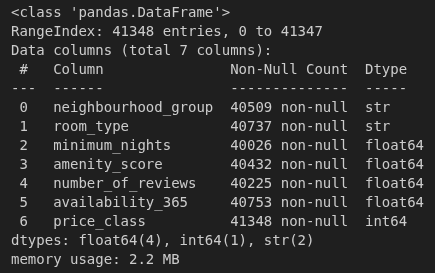
\includegraphics[scale=0.5]{figs/info-out.png}
    \caption{The output of the \texttt{info} function describing the dataset.}
  \end{figure}
  Once the data is understood, the next priority is to handle the missing values in the dataset appropriately.
  \begin{table}[H]
    \centering
    \caption{Data Imputation Strategy for Each Feature in the Dataset}
    \begin{tabularx}{\textwidth}{llX} 
        \toprule
        \textbf{Feature} & \textbf{Strategy} & \textbf{Rationale} \\
        \midrule
        \texttt{neighbourhood\_group} & Deletion & Dropping these rows avoids introducing noise into categorical spatial data. With over 40k samples remaining, the impact on dataset size is negligible.\\
        \addlinespace
        \texttt{room\_type} & Deletion & Prevents synthetic bias in a primary feature. Deletion is preferred over mode imputation to maintain the integrity of the categorical distribution.\\
        \addlinespace
        \texttt{minimum\_nights} & Median & Accounts for the "semi-categorical" nature of integer-based night stays and provides robustness against extreme outliers (skewed data).\\
        \addlinespace
        \texttt{amenity\_score} & Mean & Captures the central tendency of the scores. Since scores are typically normally distributed, the mean reflects the most representative value.\\
        \addlinespace
        \texttt{number\_of\_reviews} & Constant (0) & Missing values likely indicate a new listing with no historical activity; a constant of zero is the most logical factual replacement.\\
        \addlinespace
        \texttt{availability\_365} & Median & Protects against high variance in listing availability, ensuring the "typical" availability is captured rather than an average skewed by unbooked properties. \\
        \bottomrule
    \end{tabularx}
  \end{table}
  \pagebreak
  Now that the data is clean, analysing the class distribution is an important part of EDA that may lead to valuable insights.
  \begin{figure}[H]
    \centering
    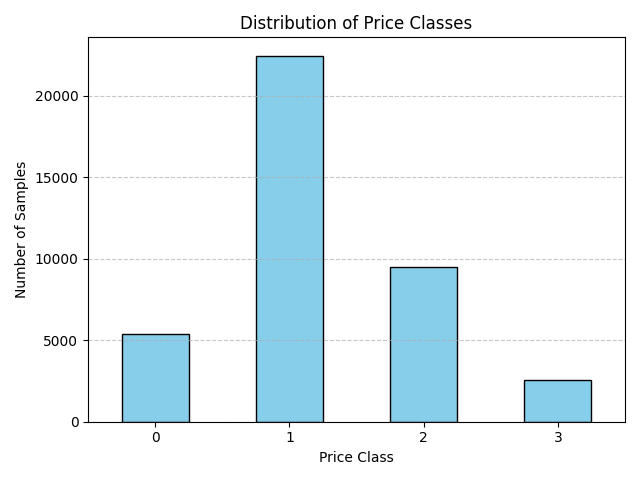
\includegraphics[scale=0.8]{figs/class_dist.png}
    \caption{A visualisation of the class distribution in the dataset.}
  \end{figure}
  \begin{table}[H]
    \centering
    \caption{Distribution of the Target Variable (\texttt{price\_class})}
    \begin{tabular}{lrr}
        \toprule
        \textbf{Price Class} & \textbf{Sample Count} & \textbf{Percentage (\%)} \\
        \midrule
        Class 0 (Budget) & 5,372  & 13.46 \\
        Class 1 (Moderate) & 22,477 & 56.33 \\
        Class 2 (Premium) & 9,502  & 23.81 \\
        Class 3 (Luxury) & 2,554  & 6.40  \\
        \bottomrule
    \end{tabular}
  \end{table}
  From the visualisations above, the imbalance is obvious and unsurprising: the 'Moderate' class takes up 56.33\% of all the listings in the dataset.\\
  The next port of call is to encode the categorical variables using an appropriate encoding scheme. The one chosen for this dataset --- specifically the \texttt{neighbourhood\_group} and \texttt{room\_type} variables --- is 'One-Hot Encoding'. The reason to use this scheme is twofold: 
  \begin{itemize}
    \item These variables have no mathematical 'ranking'. For example, Manhattan cannot be higher than Brooklyn in a way that a computer can naturally calculate without bias.
    \item Since the number of unique categories is small: 5 and 3 respectively, we can use this scheme with a much less risk of falling into the 'curse of dimensionality'.
  \end{itemize}
  The next step is is to normalize the numerical features. The method used for this dataset is Standardisation (Z-score Normalisation). Simply put, using the formula $z=\frac{x-\mu}{\sigma}$, this method shifts the data so the mean ($\mu$) is 0 and the standard deviation ($\sigma$) is 1. There are a few reasons to use this method:
  \begin{itemize}
    \item It ensures that algorithms do not get biased by the sheer magnitude of the number.
    \item It allows for faster convergence without wild oscillations in models that use Gradient Descent.
    \item It handles outliers much better than other methods like Min-Max Scaling.
  \end{itemize}
  Once the data is cleaned, split, and preprocessed; it is important to get a basic understanding of the nature of the data and whether there are any obvious identifiable patterns/consistencies in it. For the categorical features, this is done by creating a proportionate stacked bar chart.
  \begin{figure}[H]
    \centering
    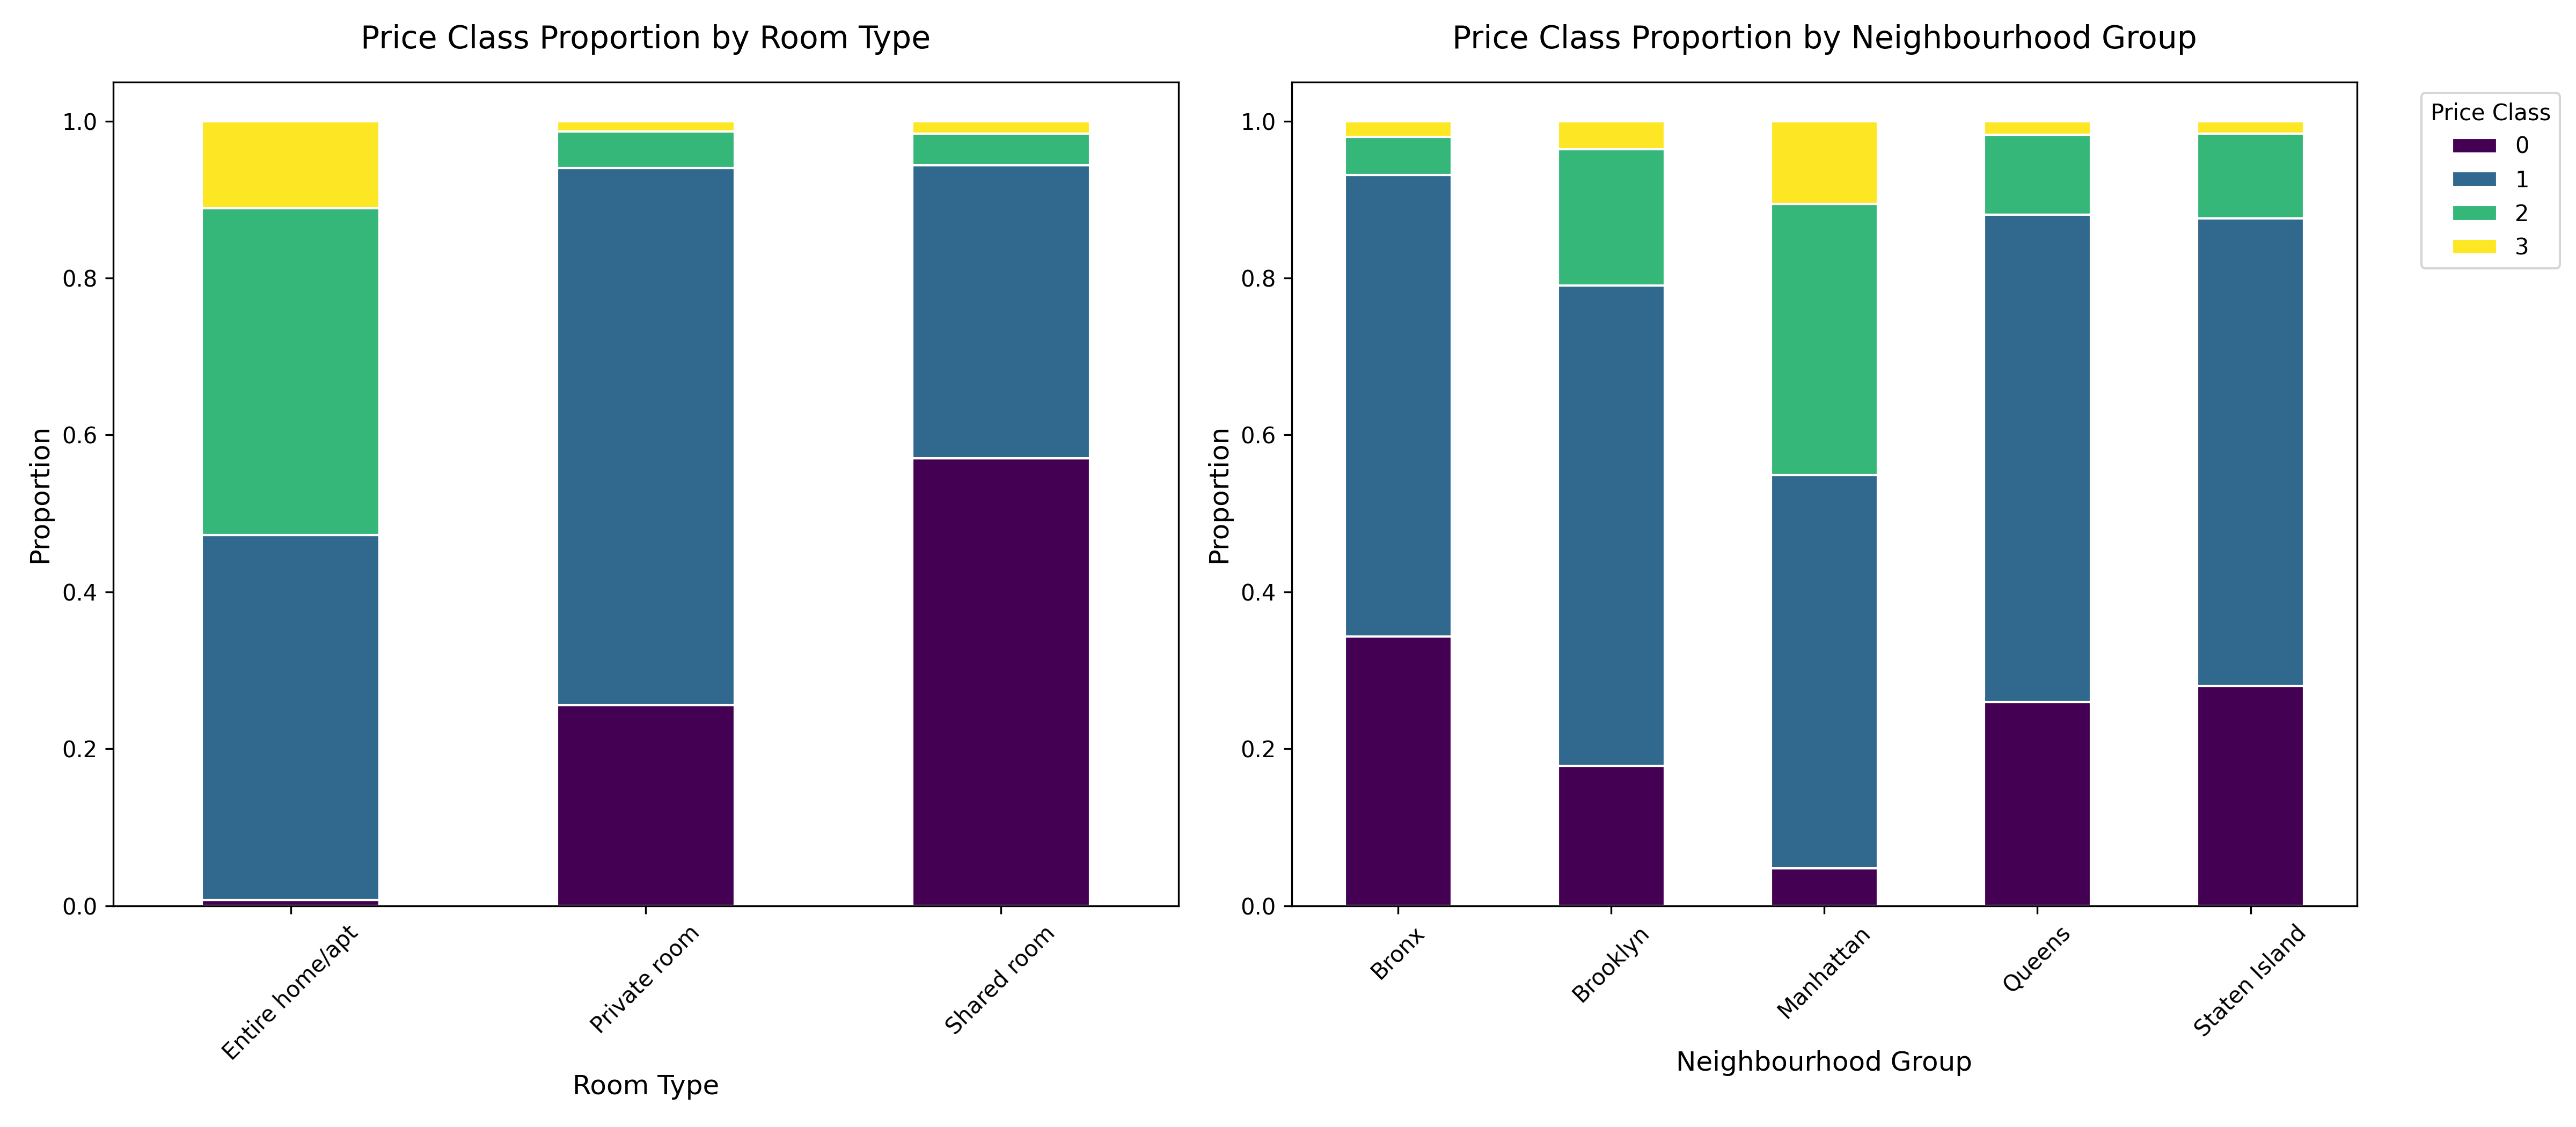
\includegraphics[scale=0.3]{figs/cat_comb_dist.png}
    \caption{A visualisation of the relationship between the categorical features and the label.}
    \label{fig:cat-dist}
  \end{figure}
  For the numerical features, this is done using box plots.
  \begin{figure}[H]
    \centering
    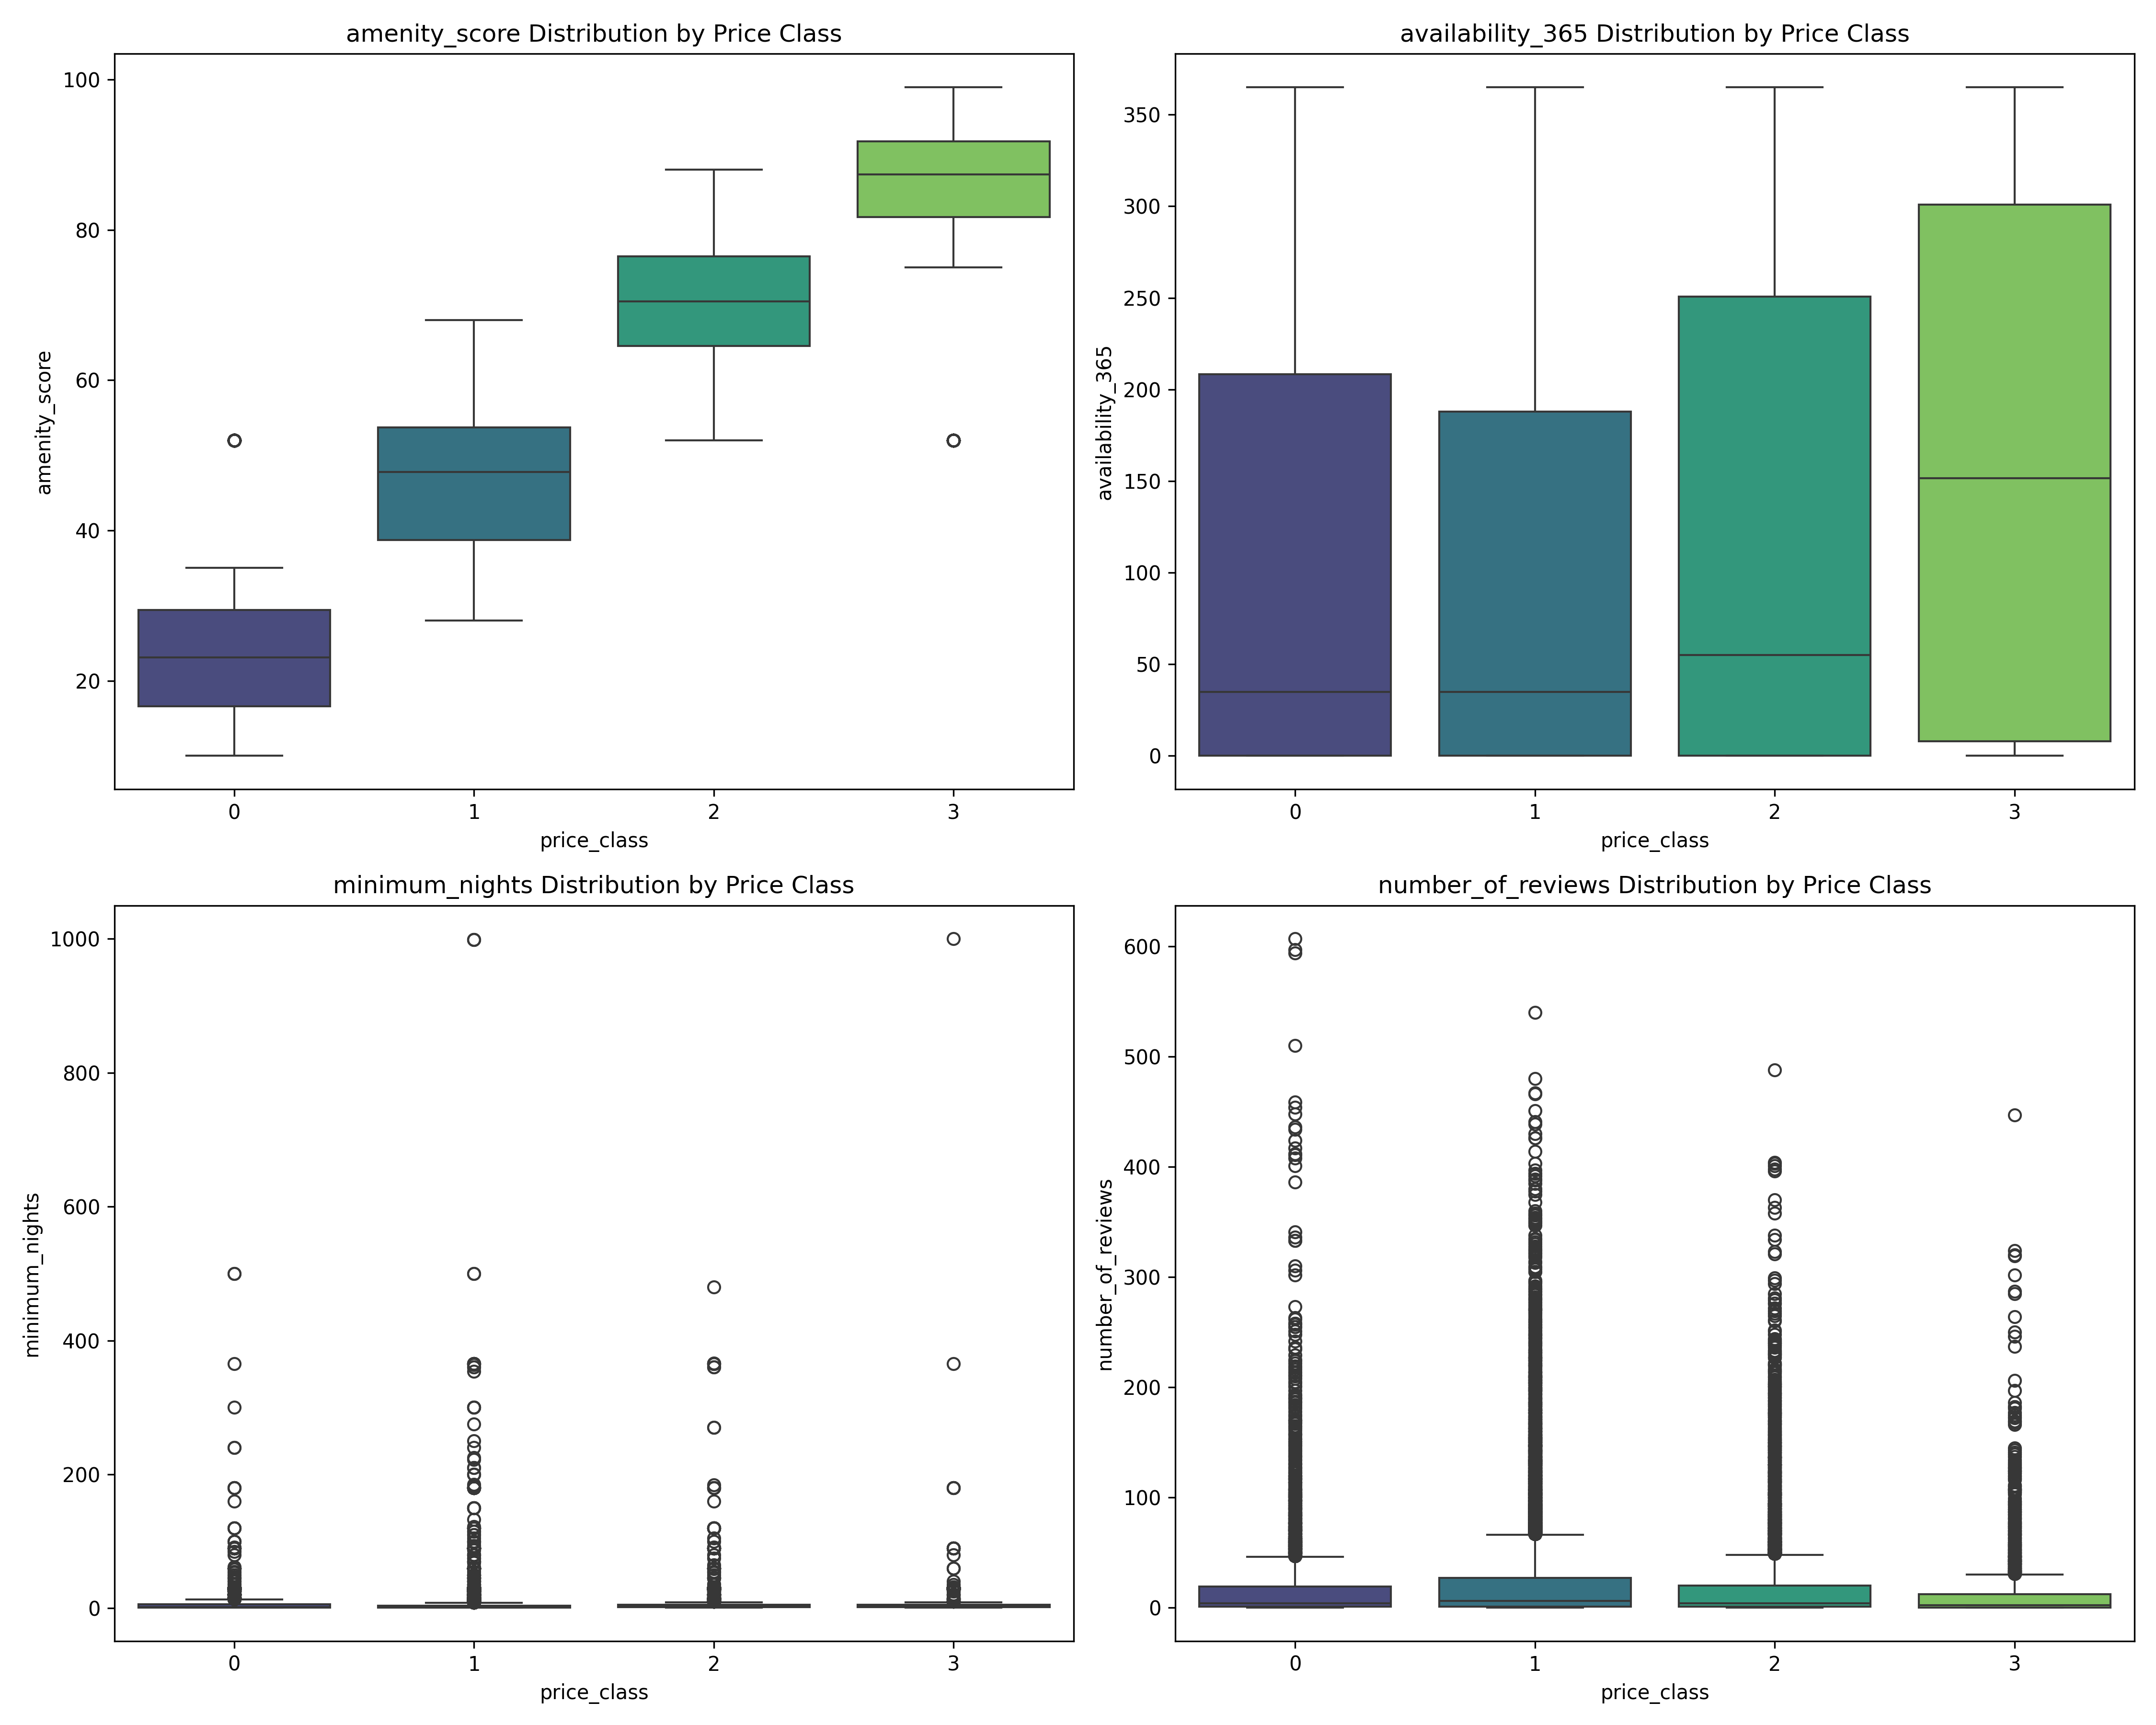
\includegraphics[scale=0.25]{figs/num_comb_dist.png}
    \caption{A visualisation of the relationship between the numerical features and the label.}
    \label{fig:num-dist}
  \end{figure}
  Understanding the correlation between features is also an important part of EDA. The correlation matrix can be visualised using a heatmap.
  \begin{figure}[H]
    \centering
    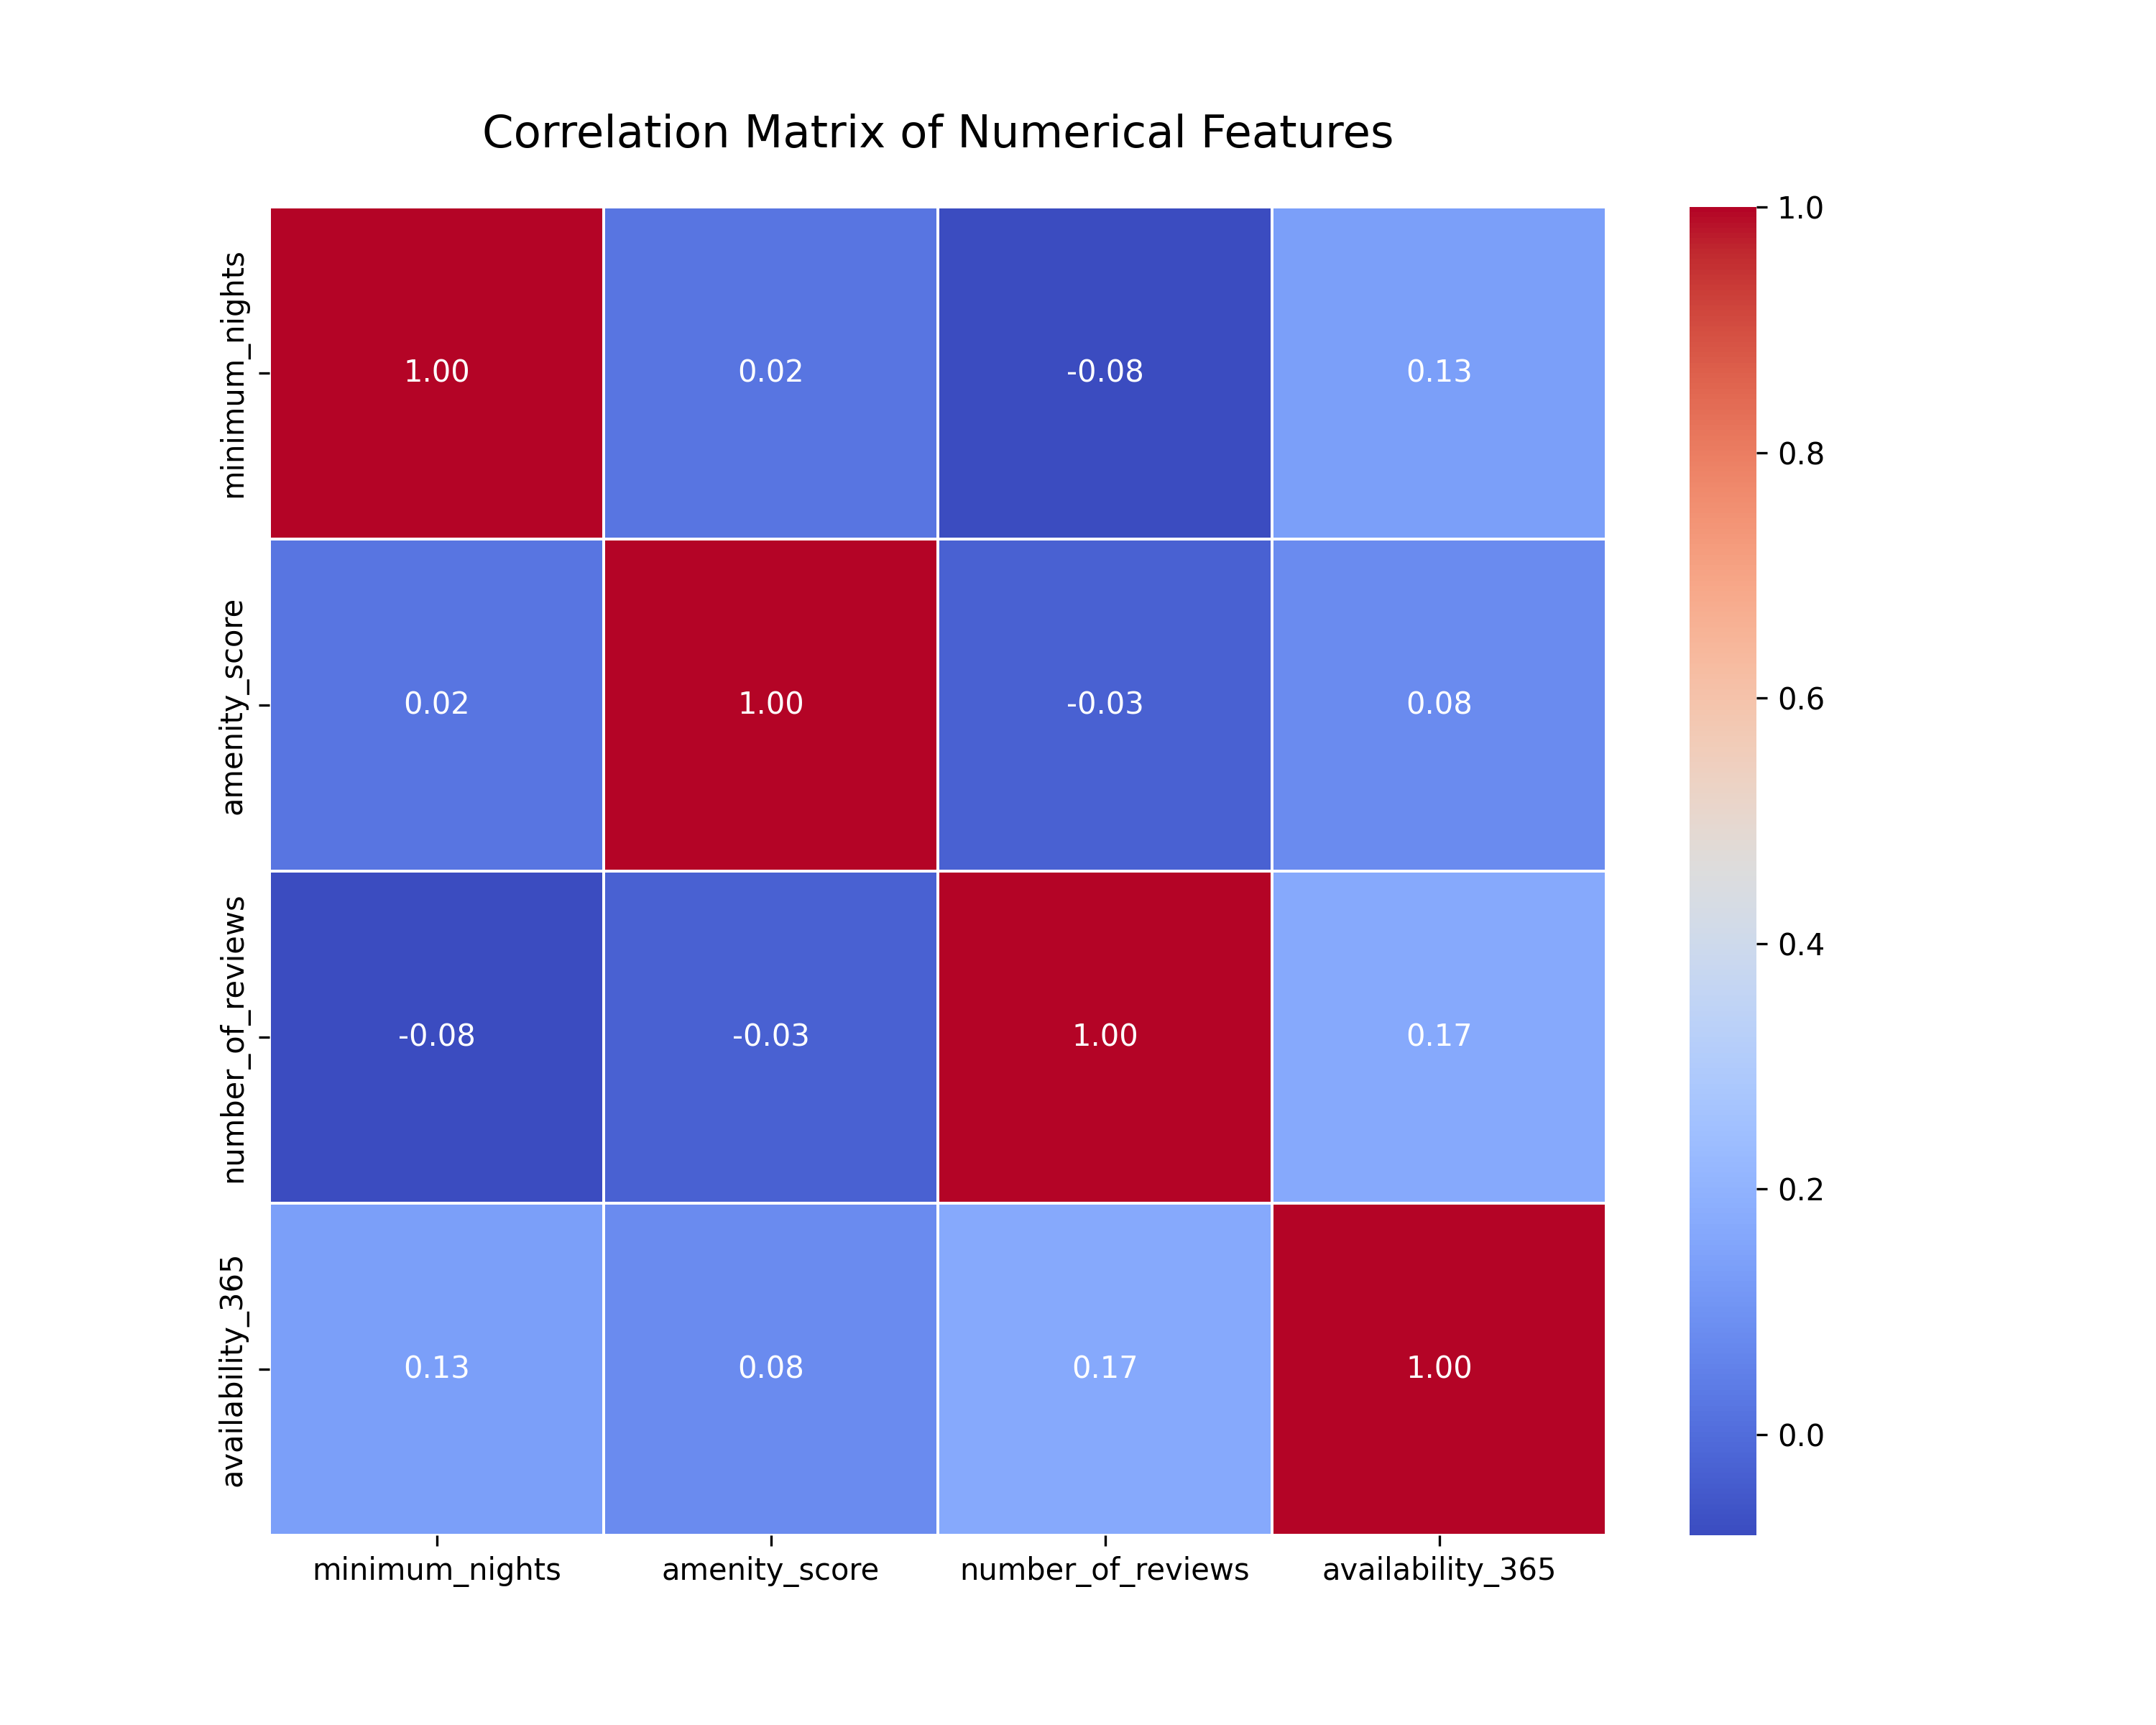
\includegraphics[scale=0.3]{figs/corr_map.png}
    \caption{Correlation matrix of numarical features visualised in a heatmap.}
  \end{figure}
  From all the available information above, there are two features that stick out: \texttt{amenity\_score} and \texttt{room\_type}. Looking at the bar chart in Figure \ref{fig:cat-dist}, it is apparent that more than 90\% of listings in class 2 and 3 fall under 'Entire home/apartment' room type. Additionally, looking at the box plots in Figure \ref{fig:num-dist}, the amenity score almost perfectly seperates each price class. Therfore, it stands to reason that the amenity score feature will be both unusually predictive and suspiciously dominant.\\[1em]
  {\large\textbf{Part B(a): Two-Layer Perceptron Implemented from Scratch}}\\
  A two-layer perceptron was impemented from scratch using only \texttt{NumPy} operations. After programming the \texttt{FFNN} class and defining a \texttt{train} function that performed all the necessary steps required to train a simple neural network, there were still a lot of issues/obstacles that needed to be ironed out. There were multiple tweaks and trial runs before the parameters were set on something that worked for the required task at hand. These are listed below:
  \begin{enumerate}
    \item \textbf{The size of the hidden layers:} After multiple trial runs, it was apparent that the required number of neurons in the hidden layer did not need to be an extravagant amount. At the end, each hidden layer ended up with 16 neurons.
    \item \textbf{The number of iterations:} Since the learning rate was kept constant (0.1) throughout the training experiments, the number of iterations needed to be sure that both models would ultimately converge was 1000.
    \item \textbf{The initialisation of the weights:} After running the training with random initialisation, the models kept falling into the vanishing gradient problem. To avoid this, after some research online, 'He' initialisation was used for the ReLU model whereas 'Xavier' initialisation was used for the sigmoid model.
  \end{enumerate}
  Once all the details were satisfactory, a final training was done which returned the following accuracies:
  \begin{table}[H]
    \centering
    \caption{Final Training and Validation Accuracies for the Sigmoid and ReLU Models}
    \begin{tabular}{lrr}
        \toprule
        \textbf{Model} & \textbf{Training Accuracy (\%)} & \textbf{Validation Accuracy (\%)} \\
        \midrule
        \textbf{Sigmoid} & 77.29 & 77.07 \\
        \textbf{ReLU} & 83.36 & 83.10 \\
        \bottomrule
    \end{tabular}
  \end{table}
  The plot for the gradients of both the models is also shown below.
  \begin{figure}[H]
    \centering
    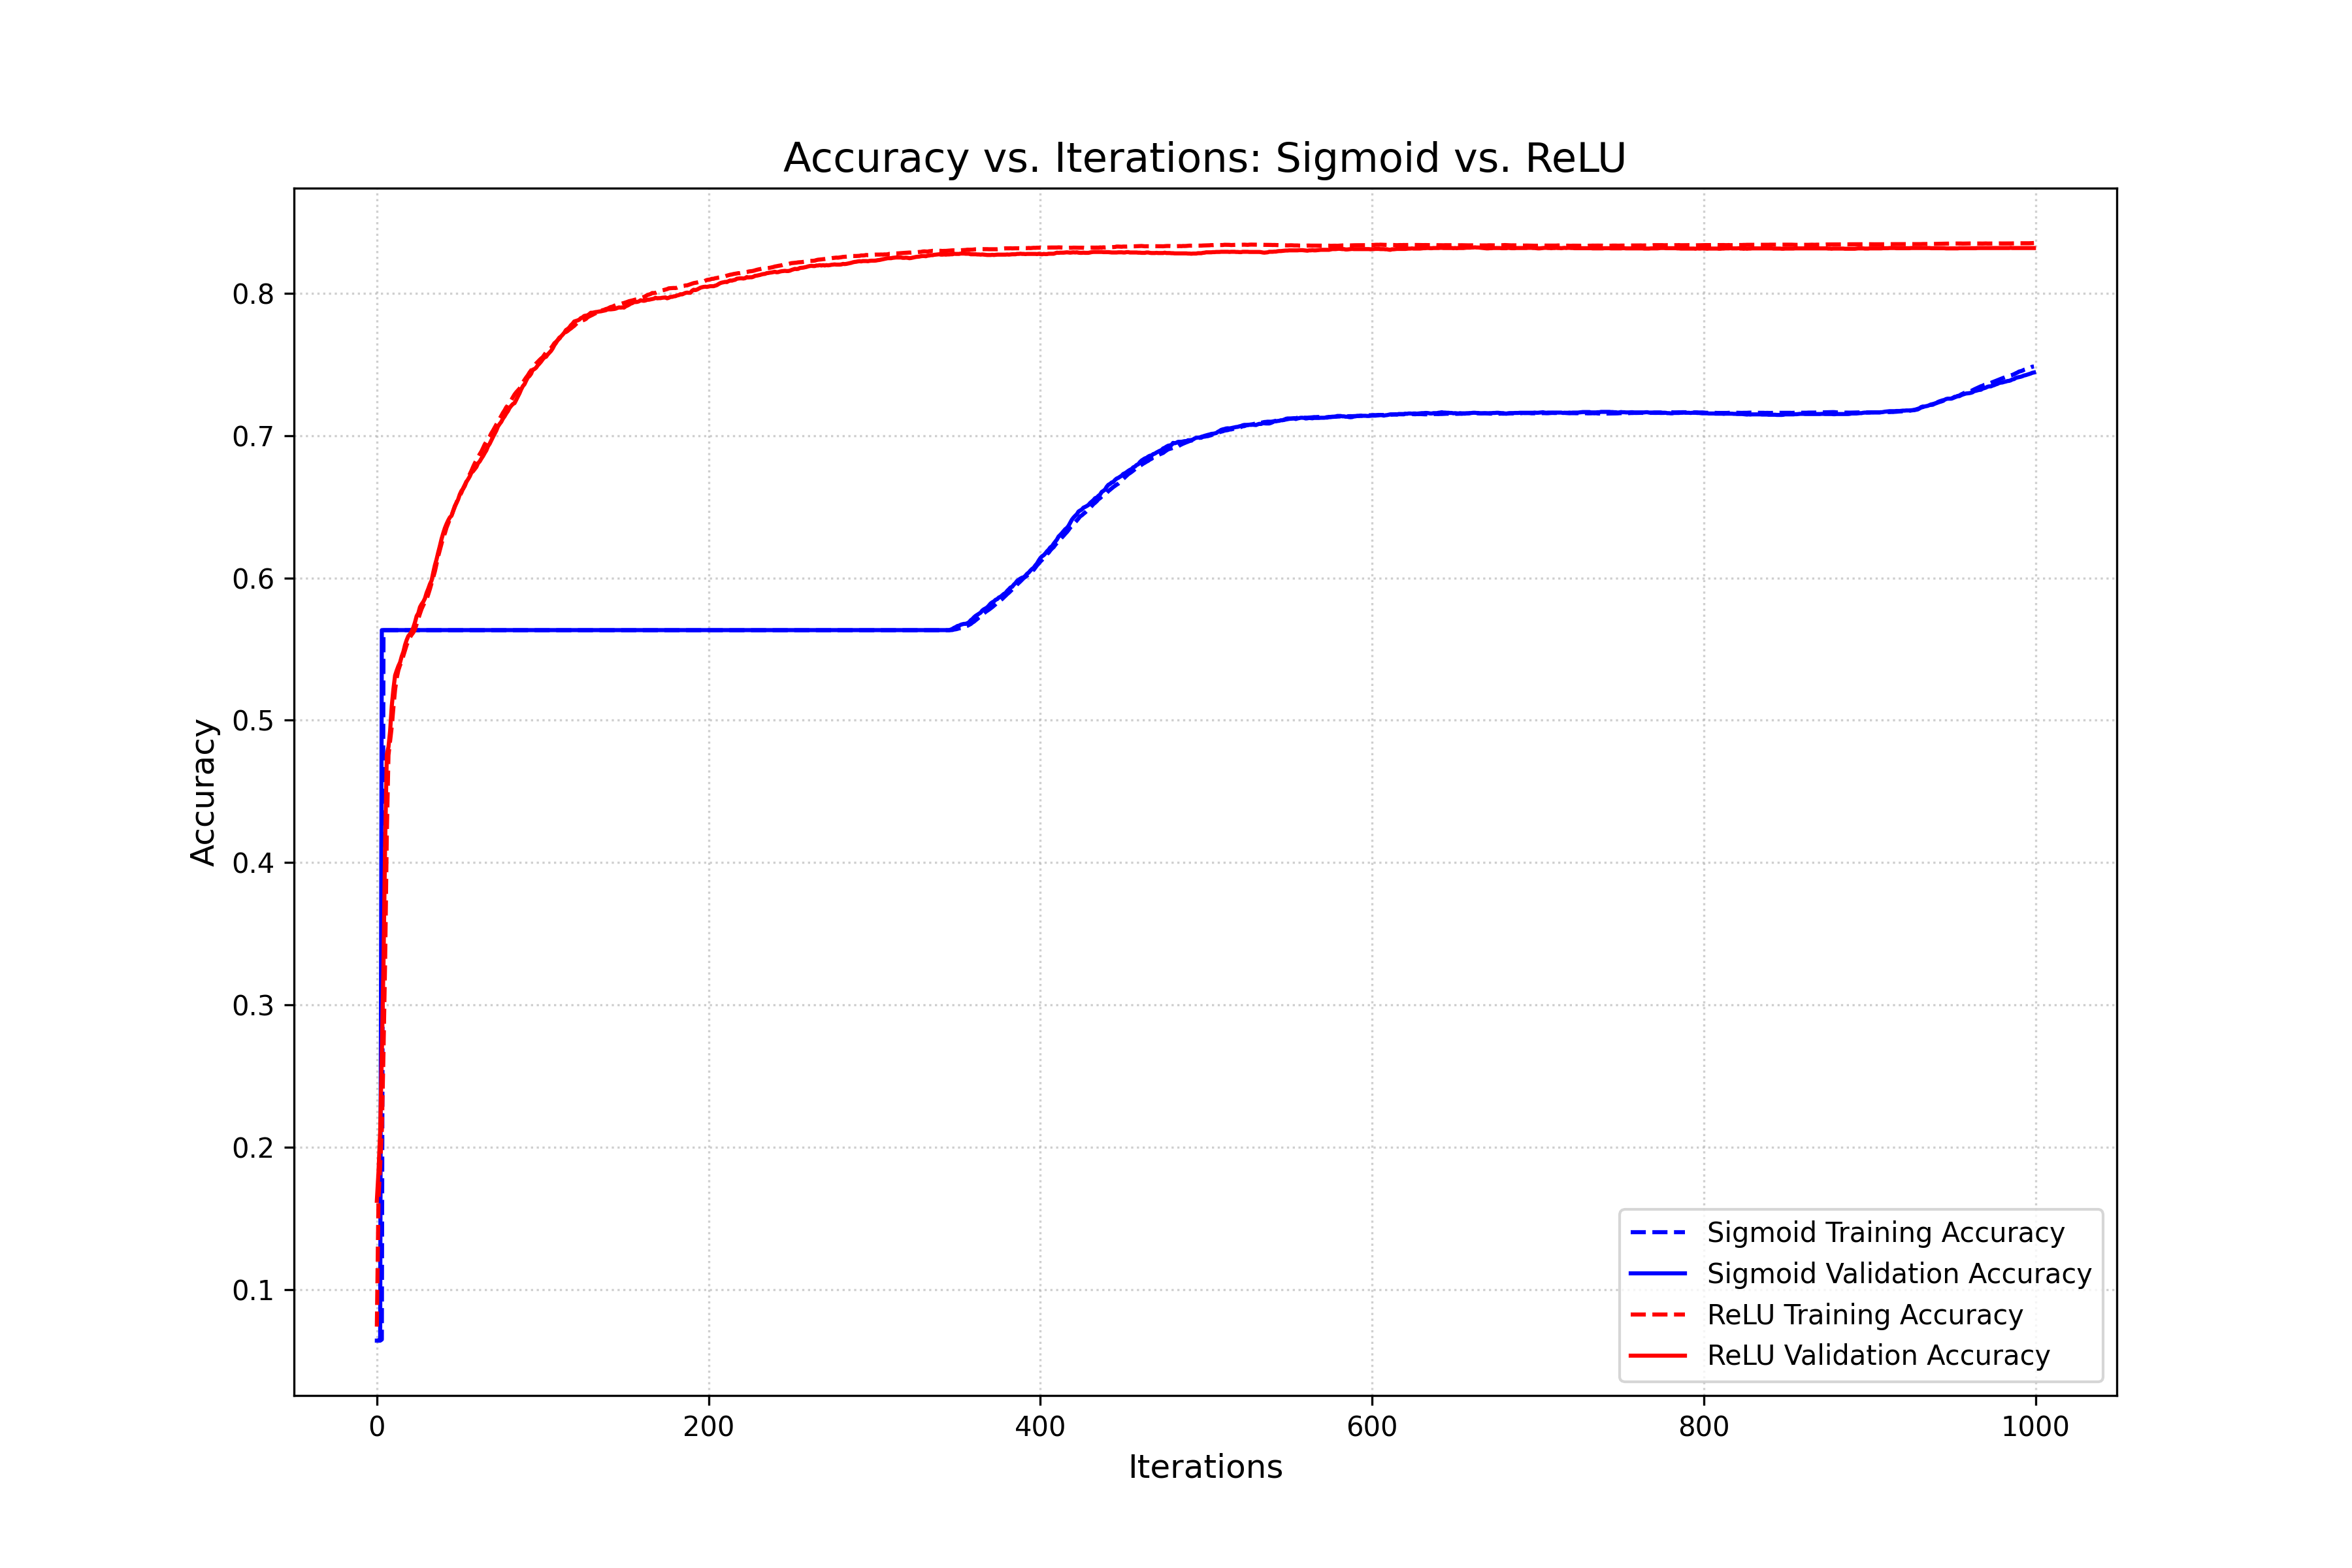
\includegraphics[scale=0.3]{figs/acc_comp.png}
    \caption{The accuracies of the models as a function of the number of iterations.}
  \end{figure}
  {\large\textbf{Part B(b): Gradient Magnitude Comparison Across Layers}}\\
  To analyze the internal learning dynamics and the "health" of the gradient flow, the average absolute magnitude of the gradients for the first hidden layer weights ($\delta W^{(1)}$) and the second hidden layer weights ($\delta W^{(2)}$) were tracked over 1000 iterations.
  \begin{figure}[H]
    \centering
    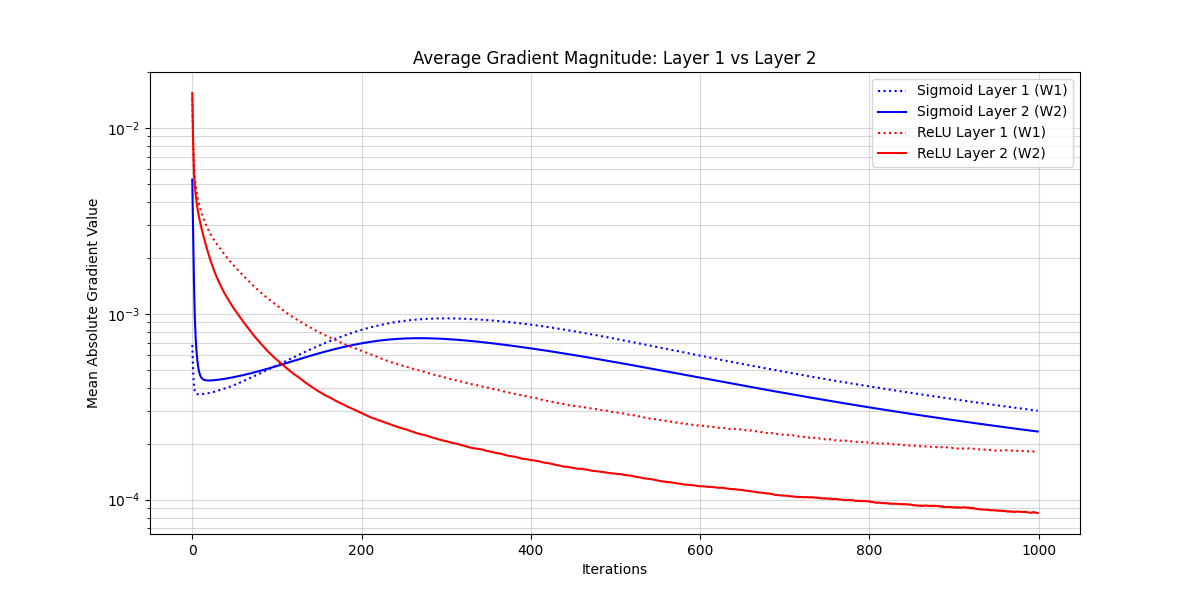
\includegraphics[scale=0.3]{figs/grad_flow_comp.png}
    \caption{The average gradient magnitude of the hidden layers as a function of the number of iterations.}
  \end{figure}
  The following trends were observed during the optimisation process for both activation functions:
  \begin{itemize}
    \item The sigmoid gradient magnitudes exhibited a distinct curve. Initially, magnitudes dropped sharply, followed by a temporary increase as weights moved into the active regions of the Sigmoid curve, and finally, a steeper decrease toward the end of the iterations. Notably, the gradients for Layer 1 were consistently slightly larger but decreased and increased more aggressively than Layer 2 at the start of the training.
    \item The gradients for ReLU started with significantly higher magnitudes than Sigmoid. While they decreased over time, the decrease was gradual and eventually plateaued. In this network, Layer 1 gradient magnitudes remained slightly higher than Layer 2, but both layers moved with stable, non-vanishing signals.
  \end{itemize}
  These results reveal several insights into the optimization of deep neural networks:
  \begin{itemize}
    \item The slightly steeper final decline in Sigmoid gradients compared to ReLU might be demonstrative of the vanishing gradient problem. Although the decline is not extreme in this specific architecture, the multiplicative effect of the Sigmoid derivative (capped at $0.25$) inherently attenuates the error signal more than ReLU's constant $1.0$ derivative.
    \item Sigmoid's initial drop followed by the surge is indicative weights transitioning through different regions of the S-curve; the final steady decrease suggests the model is approaching a region of lower sensitivity (saturation). ReLU's more gradual decrease indicates a more stable and preserved gradient flow throughout the training process.
    \item In both networks, Layer 1 gradients are larger than Layer 2 which is usually not the case when it comes to neural networks.
    \item ReLU's and Sigmoid's plateau signifies 'successful' convergence where the error $(\hat{y} - y)$ is minimized and updates become stable.
  \end{itemize}
  {\large\textbf{Part C(a): Gradient-Based Feature Attribution (Analytical)}}\\
  In the architecture studied, the forward pass begins with the input $x=x^{(0)}$. The relationship between the input and the first hidden layer's pre-activation $a^{(1)}$ is defined as:
  $$a^{(1)}=W^{(1)}x^{(0)}+b^{(1)}$$
  This is important to point out since the the loss $\mathcal L$ only depends on $\mathbf{x}$ through the first layer pre-activations. To find $\frac{\partial\mathcal L}{\partial\mathbf{x}}$, the chain rule is applied:
  $$\frac{\partial\mathcal L}{\partial\mathbf{x}}=\frac{\partial\mathcal L}{\partial a^{(1)}}\cdot\frac{\partial a^{(1)}}{\partial\mathbf{x}}$$
  $$\frac{\partial\mathcal L}{\partial\mathbf{x}}=\frac{\partial\mathcal L}{\partial a^{(1)}}\cdot (W^{(1)})^\top$$
  The notes also say that the first term on the right hand side of the above equation equals $\vec{\delta}^{(1)}$ which is obtained through the standard backward pass recursion.
  $$\frac{\partial\mathcal L}{\partial\mathbf{x}}=(W^{(1)})^\top\cdot\vec{\delta}^{(1)}$$
  The pseudocode (algorithmic steps) that outlines the analytical computation of gradients with respect to each input feature is provided below as well as how the magnitude of these gradients can be used to rank feature importance.
  \begin{algorithm}[H]
  \caption{Gradient-Based Feature Attribution}
  \begin{algorithmic}[1]
    \Procedure{FEATURE\_ATTRIBUTION}{$\{\vec{x}_k, y_k\}_{k=1}^N, W, \vec{b}$}
    \State Initialize importance vector $\vec{I}$ of size $M$
    \For{$k = 1$ \textbf{to} $N$} 
    \State FORWARDPASS($\mathbf{x}$)
      \State $\vec{\delta}^{(L)} \gets \frac{\partial L}{\partial \vec{x}^{(L)}} \odot g_L'(\vec{a}^{(L)})$
      \For{$l = L$ \textbf{down to} $2$}
        \State $\vec{\delta}^{(l-1)} \gets (W^{(l)\top} \vec{\delta}^{(l)}) \odot g'(\vec{a}^{(l-1)})$
      \EndFor
      \State $\vec{G}^{(k)} \gets W^{(1)\top} \vec{\delta}^{(1)}$        
      \For{$i = 1$ \textbf{to} $M$}
        \State $\vec{I}_i \gets \vec{I}_i + \frac{1}{N} |G_i^{(k)}|$
      \EndFor
    \EndFor
    \State \Return the importance vector sorted descendingly
    \EndProcedure
  \end{algorithmic}
  \end{algorithm}
  To justify this from an optimisation perspective, the magnitude $\left|\frac{\partial\mathcal L}{\partial\mathbf{x}}\right|$ is a meaningful measure because it represents the sensitivity of the network's loss to each feature. This implies that features with larger gradient magnitudes are those that have the most significant influence on the loss function, identifying them as the most 'informative' inputs for the model's current state.\\[1em]
  {\large\textbf{Part C(b): Implementation and Results}}\\
  To implement this feature attribution in the current architecture of the FFNN that was created, the simple solution is to just add a line of code to the backpropagation algorithm and then create a function that determines the feature relevance by aggregating the absolute magnitude of input gradients exclusively over correctly classified training instances. This approach ensures that the identified influential features are those that contribute to the model’s successful decision-making process. Since the backpropagation algorithm already calculates all the required values for the calculation, the importance vector containing the feature gradients can simply be calculated and stored in it. Once the training was done, the results are quite similar to what was expected in Part A.
  \begin{table}[H]
    \centering
    \caption{Ranked Influential Features based on Gradient Sensitivity (Sigmoid Network)}
    \begin{tabular}{llr}
        \toprule
        \textbf{Rank} & \textbf{Feature Name} & \textbf{Sensitivity Magnitude} \\
        \midrule
        1 & \texttt{num\_\_amenity\_score} & 0.417094 \\
        2 & \texttt{cat\_\_room\_type\_Private room} & 0.109173 \\
        3 & \texttt{cat\_\_neighbourhood\_group\_Manhattan} & 0.068333 \\
        4 & \texttt{cat\_\_neighbourhood\_group\_Queens} & 0.042537 \\
        5 & \texttt{cat\_\_neighbourhood\_group\_Staten Island} & 0.033062 \\
        6 & \texttt{cat\_\_room\_type\_Shared room} & 0.026062 \\
        7 & \texttt{cat\_\_neighbourhood\_group\_Brooklyn} & 0.023719 \\
        8 & \texttt{num\_\_availability\_365} & 0.018158 \\
        9 & \texttt{num\_\_minimum\_nights} & 0.015609 \\
        10 & \texttt{num\_\_number\_of\_reviews} & 0.006254 \\
        \bottomrule
    \end{tabular}
  \end{table} 
  \begin{table}[H]
    \centering
    \caption{Ranked Influential Features based on Gradient Sensitivity (ReLU Network)}
    \begin{tabular}{llr}
        \toprule
        \textbf{Rank} & \textbf{Feature Name} & \textbf{Sensitivity Magnitude} \\
        \midrule
        1 & \texttt{num\_\_amenity\_score} & 0.634728 \\
        2 & \texttt{cat\_\_room\_type\_Shared room} & 0.260162 \\
        3 & \texttt{cat\_\_room\_type\_Private room} & 0.166986 \\
        4 & \texttt{cat\_\_neighbourhood\_group\_Staten Island} & 0.147451 \\
        5 & \texttt{cat\_\_neighbourhood\_group\_Manhattan} & 0.137340 \\
        6 & \texttt{cat\_\_neighbourhood\_group\_Queens} & 0.125447 \\
        7 & \texttt{cat\_\_neighbourhood\_group\_Brooklyn} & 0.110445 \\
        8 & \texttt{num\_\_minimum\_nights} & 0.074399 \\
        9 & \texttt{num\_\_availability\_365} & 0.074173 \\
        10 & \texttt{num\_\_number\_of\_reviews} & 0.046926 \\
        \bottomrule
    \end{tabular}
\end{table}  In both architectures, \texttt{num\_\_amenity\_score} emerges as the primary driver of the model's output, exhibiting the highest aggregate sensitivity. The significantly higher sensitivity magnitudes observed in the ReLU network are attributable to ReLU's constant gradient of 1.0, which avoids the vanishing gradient decay inherent in Sigmoid's 0.25-capped derivative. While both networks align with the general findings of Part A, the ReLU network identifies \texttt{cat\_\_room\_type\_Shared room} as more influential than the Sigmoid network suggests. This shift indicates that the ReLU model has established a more sensitive decision boundary around room-sharing features, capturing non-linear relevance that was secondary in the Sigmoid analysis.\\
  The implemented algorithm is very similar to the one derived in Part C(a), as it uses the training cycle to store the feature attributes. However, the main difference is that the aggregation of the absolute gradient magnitudes is restricted specifically to correctly classified training instances.
  \begin{algorithm}[H]
  \caption{Gradient-Based Feature Attribution (According to Section 2.8 of Charu C. Aggarwal’s Textbook)}
  \begin{algorithmic}[1]
    \Procedure{FEATURE\_ATTRIBUTION}{$\{\vec{x}_k, y_k\}_{k=1}^N, W, \vec{b}$}
    \State Initialize importance vector $\vec{I}$ of size $M$
    \State $N_{correct} \gets 0$
    \For{$k = 1$ \textbf{to} $N$} 
    \State FORWARDPASS($\vec{x}_k$)
    \If{$\text{argmax}(\hat{\vec{y}}_k) == \text{argmax}(\vec{y}_k)$}
      \State $N_{correct} \gets N_{correct} + 1$
      \State $\vec{\delta}^{(L)} \gets \hat{\vec{y}}_k - \vec{y}_k$
      \For{$l = L$ \textbf{down to} $2$}
        \State $\vec{\delta}^{(l-1)} \gets (W^{(l)\top} \vec{\delta}^{(l)}) \odot g'(\vec{a}^{(l-1)})$
      \EndFor
      \State $\vec{G}^{(k)} \gets W^{(1)\top} \vec{\delta}^{(1)}$        
      \For{$i = 1$ \textbf{to} $M$}
        \State $\vec{I}_i \gets \vec{I}_i + |G_i^{(k)}|$
      \EndFor
    \EndIf
    \EndFor
    \State $\vec{I} \gets \vec{I} / N_{correct}$
    \State \Return the importance vector sorted descendingly
    \EndProcedure
  \end{algorithmic}
  \end{algorithm}
  {\large\textbf{Part D: Test Evaluation and Generalisation Analysis}}\\
  The trained models were evaluated on the provided test dataset. The reported accuracies are as follows:
  \begin{itemize}
    \item \textbf{Sigmoid Network Test Accuracy:} 40.73\%
    \item \textbf{ReLU Network Test Accuracy:} 34.40\%
  \end{itemize}
  The table below illustrates the performance gap between the datasets:
  \begin{table}[H]
    \centering
    \caption{Model Accuracy Comparison across Datasets}
    \begin{tabular}{lrrr}
        \toprule
        \textbf{Model} & \textbf{Training Acc. (\%)} & \textbf{Validation Acc. (\%)} & \textbf{Test Acc. (\%)} \\
        \midrule
        \textbf{Sigmoid} & 77.29 & 77.07 & 40.73 \\
        \textbf{ReLU} & 83.36 & 83.10 & 34.40 \\
        \bottomrule
    \end{tabular}
  \end{table}
  There is a significant generalization gap. While the models performed consistently across training and validation sets (with less than 1\% difference), they failed to generalize to the test set, with accuracy dropping by approximately 36\% for Sigmoid and 49\% for ReLU. This indicates that while the models did not "overfit" to the training noise, they failed to learn features that remain invariant across different data distributions.\\
  The failure in generalization can be traced back to the following evidence:
  \begin{itemize}
    \item \textbf{Gradient-Based Attribution (Part C):} The analysis based on Section 2.8 of the textbook revealed that the models are hyper-sensitive to the \texttt{num\_\_amenity\_score} feature. In the ReLU network, the sensitivity magnitude for this feature (0.634) was substantially higher than other features.
    \item \textbf{Exploratory Data Analysis (Part A):} The model has effectively become an "amenity score classifier" rather than a robust price predictor. If the distribution of amenity scores or their relation to price classes differs in the test set compared to the training set, the model's over-reliance on this single feature leads to categorical failure.
  \end{itemize}
  The model performs well during training because it identifies a strong mathematical correlation between the amenity score and the target within that specific data slice. However, by assigning such high sensitivity to one attribute, the model ignores the secondary predictive power of other features. As specified in the textbook, backpropagation identifies the most relevant features for classification; in this case, it highlights an unhealthy dependency on a single variable that does not hold its predictive power in the test environment.\\
  A strategy that could mitigate this is the Implementation of L2 regularization within the backpropagation update. L2 regularization penalizes large weight magnitudes. By adding this penalty, the model would be prevented from assigning the disproportionately high weights to the\\ \texttt{num\_\_amenity\_score} input that were observed in the gradient analysis. This forces the network to distribute its learned importance across multiple features, resulting in a more balanced decision boundary that is less susceptible to shifts in any single feature's distribution.
\end{question}


\begin{question}[Bias Gradients, Parameter Sharing, and Activation Effects]
  The computation graph for the FFNN in this question is shown in the image below:
  \begin{figure}[H]
    \centering
    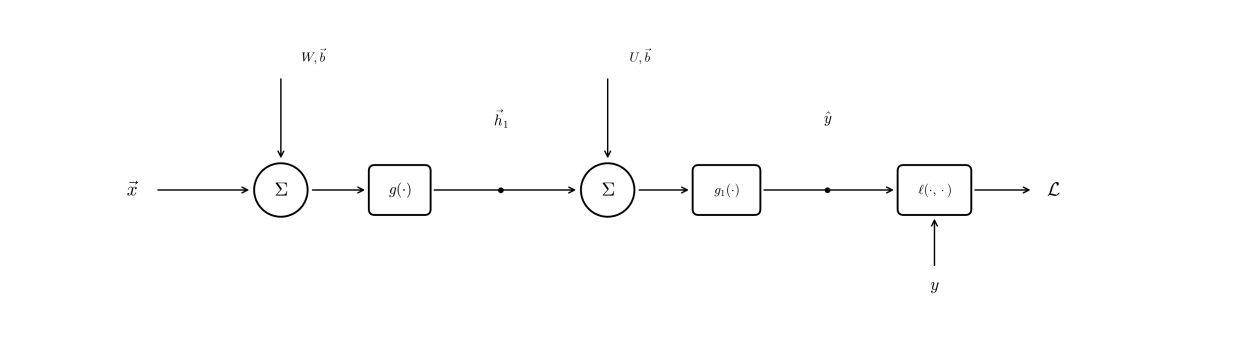
\includegraphics[scale=0.3]{figs/ffnn.png}
    \caption{Computation graph for a two-layer MLP with a shared bias parameter}
  \end{figure}
  The paths where the shared bias vector $b$ affects the loss function can be outlined by looking at the computation graph and the forward pass equations provided.\\
  The first path, where the bias directly influences the pre-activation of the output layer:
  $$L=\ell(g_1(U\mathbf{h}_1+b),y)$$
  The second path, where the bias influences the loss by first changing the representation in the hidden layer, which then flows through the rest of the network.
  $$L=\ell(g_1(U(g(W\mathbf{x}+b))+b),y)$$
  In this FFNN, when a parameter is used multiple times in the forward pass, its total gradient is the sum of the gradients calculated for each occurrence.
  From this, the backpropagation required utilises the chain rule as follows:
  $$\frac{\partial L}{\partial b}=\frac{\partial L}{\partial a^{(2)}}\cdot\frac{\partial a^{(2)}}{\partial b}+\frac{\partial L}{\partial a^{(1)}}\cdot\frac{\partial a^{(1)}}{\partial b}$$
  Starting with the direct path:
  $$\frac{\partial L}{\partial a^{(2)}}=\frac{\partial L}{\partial y}\odot g'_1(a^{(2)})=\vec{\delta}^{(2)}$$
  $$\frac{\partial a^{(2)}}{\partial b}=I$$
  Continuing with the 'indirect' path:
  $$\frac{\partial L}{\partial a^{(1)}}=(U^\top\vec{\delta}^{(2)})\odot g'_1(a^{(1)})=\vec{\delta}^{(1)}$$
  $$\frac{\partial a^{(1)}}{\partial b}=I$$
  Putting the two together:
  $$\frac{\partial L}{\partial b}=\vec{\delta}^{(2)}+\vec{\delta}^{(1)}$$
  Or, in terms of $\vec{\delta}^{(2)}$:
  $$\frac{\partial L}{\partial b}=\vec{\delta}^{(2)}+(U^\top\vec{\delta}^{(2)})\odot g'_1(a^{(1)})$$

\end{question}

\end{document}
